\documentclass{article}
\usepackage{amsmath, amssymb, kotex, hyperref, graphicx, mdframed, setspace,enumitem}
\usepackage[a4paper, margin = 40pt]{geometry}
\setstretch{1.5}
\begin{document}
\title{Arima Model - 1}
\author{강의 : 김성범 교수님\\ 정리 :  김선중}
\date{\today}
\maketitle

이것은 \href{https://youtu.be/ma_L2YRWMHI?list=PLpIPLT0Pf7IqSuMx237SHRdLd5ZA4AQwd}{ARIMA 모델 개요 - Part 1
} 강의에 대한 노트이다.
\tableofcontents

\newpage
%%
\section{정상성(stationarity)}
\begin{center}
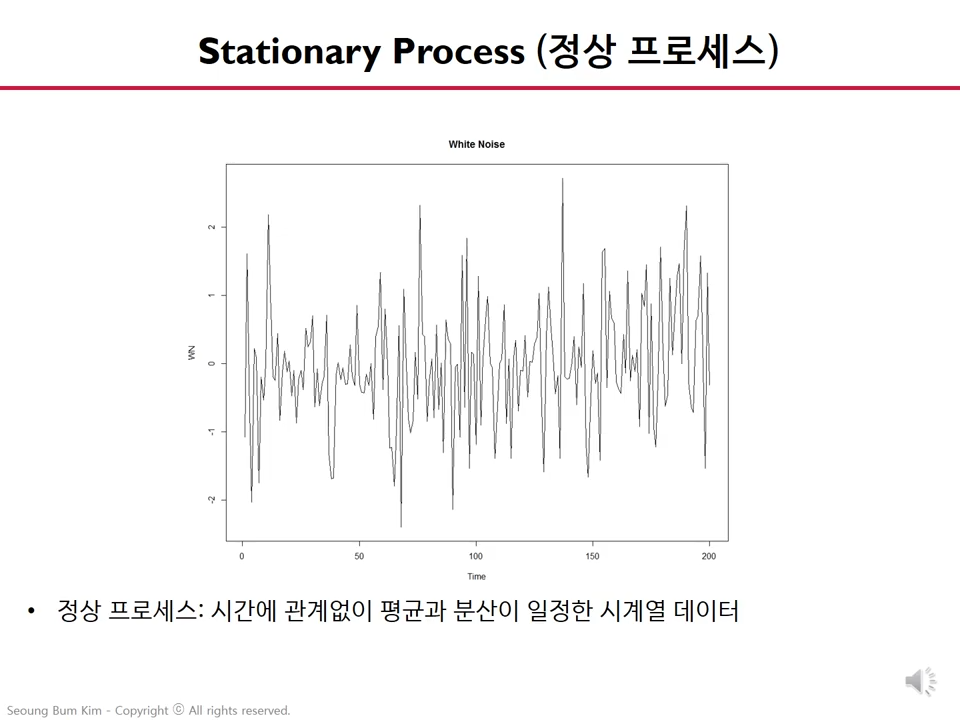
\includegraphics[width=.45\textwidth]{1stationarity_1}
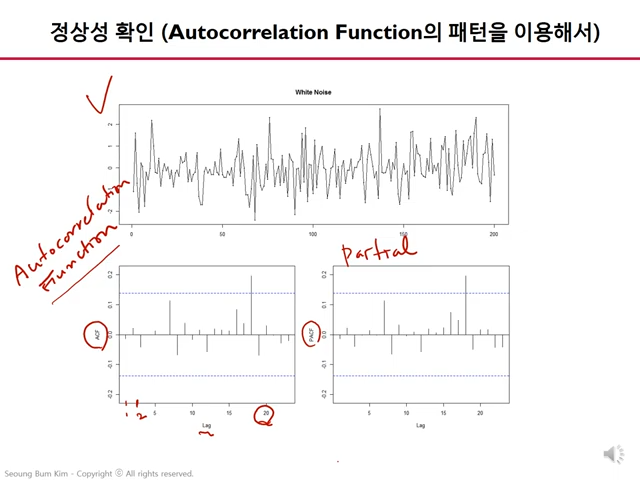
\includegraphics[width=.45\textwidth]{1stationarity_2}
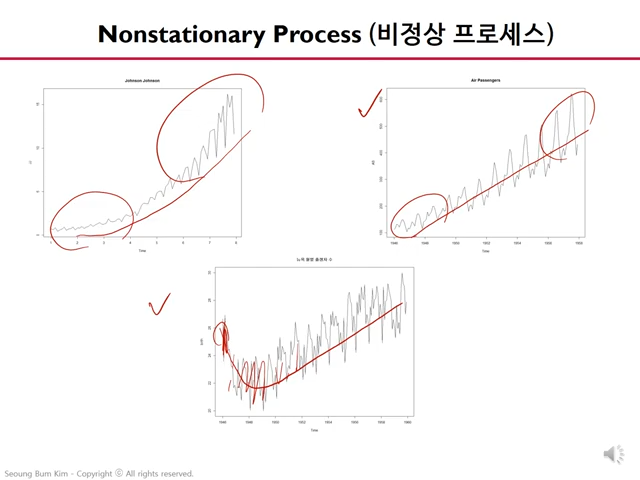
\includegraphics[width=.45\textwidth]{1stationarity_3}
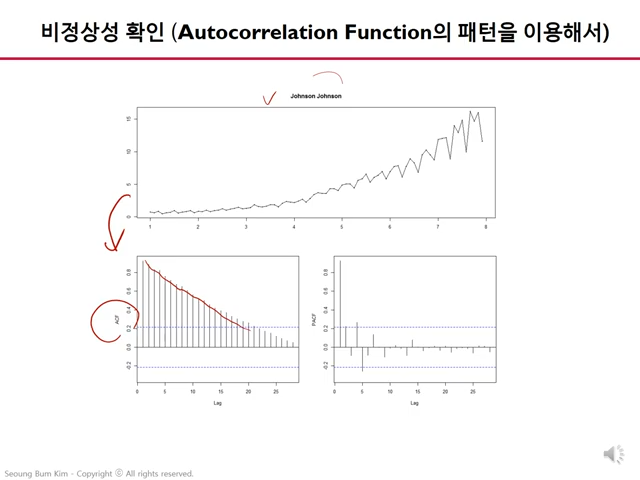
\includegraphics[width=.45\textwidth]{1stationarity_4}
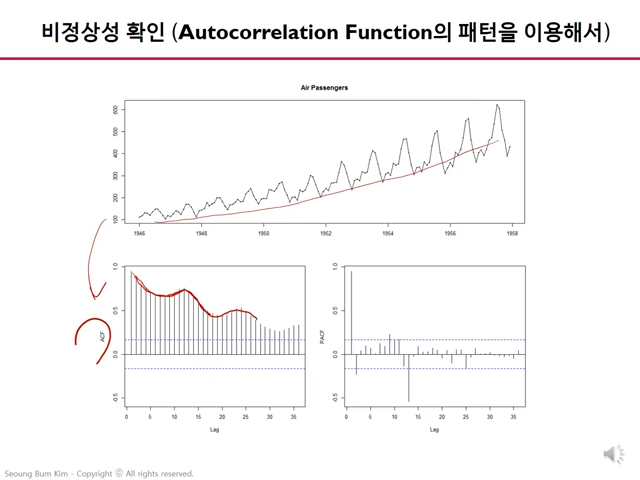
\includegraphics[width=.45\textwidth]{1stationarity_5}
\end{center}
가장 먼저 보이는 말이 `정상 프로세스(stationary process)'이다.
정상(stationary)이라는 말은 앞으로 정의할 것이지만, 프로세스(과정, proces)에 대해서는 언급이 없어서, 여기에 설명해보았다.
확률과정(stochastic function)이란, 어떤 확률공간 \((\Omega, \mathcal F, P)\)에 대한 확률변수(random variable)들의 집합을 말한다.
\footnote{\url{https://en.wikipedia.org/wiki/Stochastic_process}}
\[\{X(t):t\in T\}\]
많은 경우에 \(t\)는 시간을 뜻하는 인덱스이다.
그리고 지금은 정말로 `시계열' 데이터를 다루고 있기 때문에 \(t\)를 시간이라고 봐도 괜찮다.

이러한 확률과정들 중에 정상 확률과정이란, (강의에 따르면) 시간에 관계없이 평균과 분산이 일정한 데이터를 뜻한다.
반면, Shumway의 책에 따르면 stationarity는 다음 두 가지의 서로다른 정의가 있다.
원문을 그대로 가져와보았다.

(Definition)
A \emph{strictly stationary} time series is one for which the probabilistic behavior of every collection of values
\[\{x_{t_1},x_{t_2},\cdots,x_{t_k}\}\]
is identical to that of the time shifted set
\[\{x_{t_1+h},x_{t_2+h},\cdots,x_{t_k+h}\}\]
That is, 
\[P\{x_{t_1}\le c_1,\cdots x_{t_k}\le c_k\}=P\{x_{t_1+h}\le c_1,\cdots x_{t_k+h}\le c_k\}\tag{1.19}\]
for all \(k=1,2,\cdots\) all time points \(t_1,t_2,\cdots,t_k\), all numbers \(c_1,c_2,\cdots c_k\) and all time shift \(h=0,\pm1,\pm2,\cdots\).

If a time series is strictly stationary, then all of the multiplicative distribution function for subsets of variables must agree with their counterparts in the shifte set of all values of the shift parameter \(h\).
For example, when \(k=1\), (1.19) implies that
\[P\{x_s\le c\}=P\{x_t\le c\}\tag{1.20}\]
for any time points \(s\) and \(t\).
This statement implies, e.g., that the probability the value of a time series sampled hourly is negative at 1 AM is the same as at 10 AM.
In addition, if the mean function, \(\mu_t\), of the series \(x_t\) exists, (1.20) implies \(\mu_s=\mu_t\) for all \(s\) and \(t\), and hence \(\mu_t\) is must be constant;
\[\mu_s=\int_u uf_s(u)\,du=\int_u uf_t(u)\,du=\mu_t\]
where \(f_t\) and \(f_s\) are the derivatives of \(P\{x_s\le c\}\) and \(P\{x_s\le c\}\), resepectively, with respect to \(c\).

Note, e.g., that a random walk process with drift is not strictly stationary because its mean function changes with time.

When \(t=2\), we can write (1.19) as
\[P\{x_s\le c_1,x_t\le c_2\}=P\{x_{s+h}\le c_1, x_{t+h}\le c_2\}\tag{1.21}\]
for any time points \(s\) and \(t\) and ahift \(h\).
Thus, if the variance function of the process exists, (1,21) implies that the autocovariance of the series \(x_t\) satisfies
\begin{align*}
\gamma(s,t)
&=E[(x_s-\mu_s)(x_t-\mu_t)]\\
&=\iint_{u,v}(u-\mu)(v-\mu)f_{t,s}(u,v)\,dudv\\
&=\iint_{u,v}(u-\mu)(v-\mu)f_{t+h,s+h}(u,v)\,dudv\\
&=E[(x_{s+h}-\mu_{s+h})(x_{t+h}-\mu_{t+h})]=\gamma(s+h,t+h).
\end{align*}
for all \(s\) and \(t\) and \(h\).
We may interpret this result by saying the autocovariance function of the process depend only on the time difference between \(s\) and \(t\), and not on the actual times.

The version of stationarity in (1.19) is too strong for most applications.
Moreover, it is difficult to assess strict stationarity from a single dataset.
Rather than impose conditions on all possible distributions of a time series, we will use a milder version that imposes conditions only on the first two moments of the series.
We now leave the following definition

(Definition)
A \emph{weakly stationary} time series, \(x_t\), is a finite variance process such that
\begin{enumerate}
\item[(i)]
the mean value function, \(\mu_t\), defined in (1.11) is constant and does not depend on time \(t\), and
\item[(ii)]
the covariance function, \(\gamma(s,t)\) defined in (1.12) depends on \(s\) and \(t\) only through their difference \(|s-t|\).
\end{enumerate}
Henceforce, we will use the term stationary, to mean weak stationarity;
if a process is stationary, in the strict sence, we will use the term strictly stationary.

It should be clear from the discussion of strict stationarity following the first definition that a struct stationary, finite variance, time series is also stationary.
The converse is not true unless there are further conditions.

두번째 캡쳐에서는 어떤 시계열에 대한 ACF(autocorrelation function) 그래프를 그리고 있다.
이 그림에 대한 설명은 추후에 자세히 할 예정이라고하지만, 어쨌든 현재 상황에서도 해석할 수 있을 듯하다.
%특정한 시각 \(t\)를 정하고, 그 시각에서 일정한 만큼의 timestep \(h\)를 정할 수 있다.
%즉
%\[\{X_t, X_{t+1},\cdots,X_{t+h}\}\]
%와 같이 생긴 확률변수들의 수열을 생각할 수 있다.
%그리고, 각각의 lag \(l<h\)에 대하여, 새로운 확률변수들의 수열
%\[\{X_{t+l}, X_{t+l+1},\cdots,X_{t+l+h}\}\]
%을 고려하고 두 확률변수가 일치하는 
Shumway의 책에서는 다음과 같이 autocorrelation을 정의한다.

(Definition) The \emph{autocovariance function} of a stationary times series will be written as
\[\gamma(h)=E[(x_{t+h}-\mu)(x_t-\mu)]\tag{1.24}\]
(Definition) The \emph{autocorrelation function} (ACF) of a stationary time series will be written as
\[\gamma(h)=\frac{\gamma(t+h,t)}{\sqrt{\gamma(t+h,t+h)\gamma(t,t)}}=\frac{\gamma(h)}{\gamma(0)}\]
이 식에서 \(h\)는 lag를 의미할 것이다.

두번째 캡쳐에서의 두번째 그림은, PACF(partial autocorrelation function)의 그래프가 나타나고 있다.
어떤 시계열이 stationary한지를 판단하는 정성적인 기준은 다음과 같다.
ACF 그래프가 특정한 패턴이 없이 임의로 나타나는 경우에는 station

세번째 캡쳐의 시계열들은 시간이 흐름에 따라서 평균과 분산이 계속 바뀌고 있다.
따라서 non-stationary time series이다.

네번째 캡쳐의 시계열 또한 non-stationary해보인다.
ACF가 감소하는 모습을 보이므로 non-stationary하다고 말한다.

다섯번째 캡쳐 또한 non-stationary하다.
이 시계열 또한 ACF가 (약간의 fluctuation이 있다고는 해도) 대체로 감소하는 경향을 보이므로 non-stationary하다고 말한다.


%%
\section{AR, MA}
\begin{center}
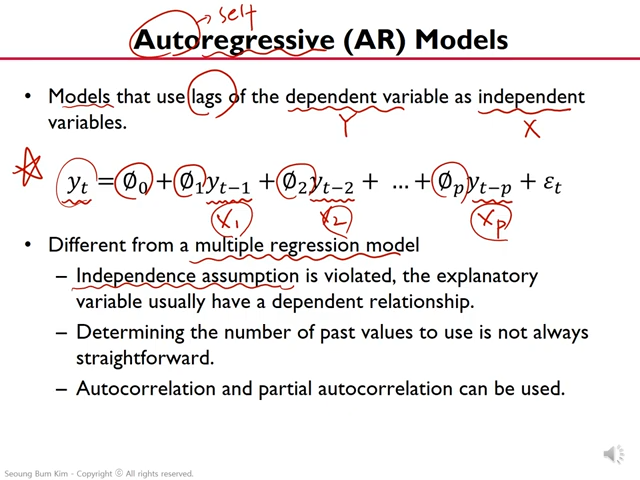
\includegraphics[width=.45\textwidth]{2ARMA_1}
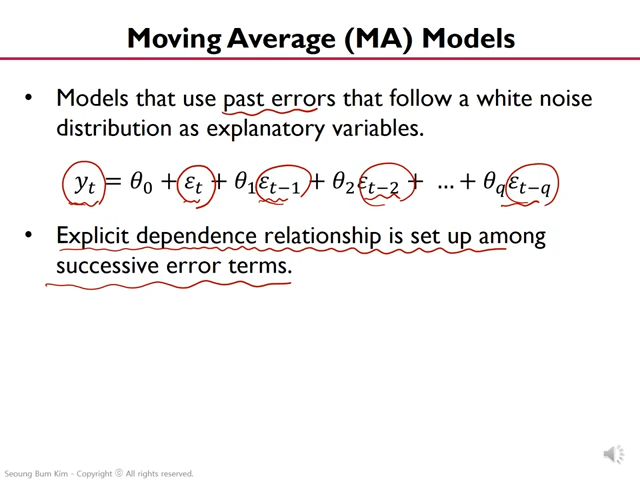
\includegraphics[width=.45\textwidth]{2ARMA_2}
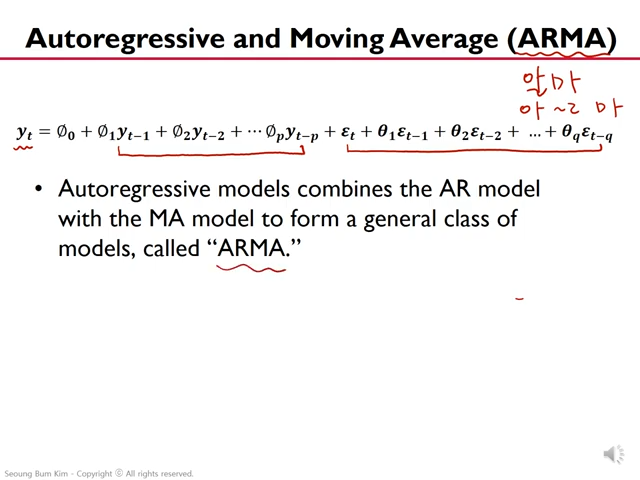
\includegraphics[width=.45\textwidth]{2ARMA_3}
\end{center}

%
\subsection{AR model}
이러한 데이터를 모델링하는 방법으로, AR 모델 (autoregressive model)을 사용한다.
autoregressive라고 함은, 자기 자신(의 이전 timestep)을 가지고 현재의 자기 자신($y_t$)을 예측한다는 뜻이다.
정확하게는 \(y_t\)를 \(y_{t_1}\), \(y_{t_2}\), \(\cdots\), \(y_{t_p}\)들의 linear combination으로 예측한다.
\[y_t = \phi_0+\phi_1y_{t-1}+\phi_2y_{t-2}+\cdots+\phi_py_{t-p}+\epsilon_t\]

강의에서, AR 모델은 다변수 회귀와는 다르다고 말하고 있는데 주요한 점들은 다음과 같다.
\begin{itemize}
\item
변수들 간의 독립성이 보장되지 않는다.
\item
\(p\)값을 직접 정해야 한다.
\item
ACF와 PACF가 사용될 수 있다.
\end{itemize}

%
\subsection{MA model}
이번에는 \(y_{t-i}\)들이 아닌 error terms, 즉 \(\epsilon_{t-i}\)들의 linear combination으로 \(y_t\)를 예측하는 방법이 있다.
이것을 moving average 방법이라고 한다.
\[y_t = \theta_0\epsilon_t+\theta_1y_{t-1}+\phi_2y_{t-2}+\cdots+\phi_qy_{t-q}\]

그런데 도저히, 이것이 왜 moving average라고 불리는 지 모르겠다.
기존에 알고 있던 `이동평균'의 개념과 전혀 일치하지 않아 보인다.

%
\subsection{ARMA model}
AR model과 MA model을 결합하면 ARMA model을 만들 수 있다.
\[y_t = \phi_0+\phi_1y_{t-1}+\phi_2y_{t-2}+\cdots+\phi_py_{t-p}+\theta_1\epsilon_{t-1}+\phi_2\epsilon_{t-2}+\cdots+\phi_q\epsilon_{t-q}\]

%%
\section{ARIMA}
\begin{center}
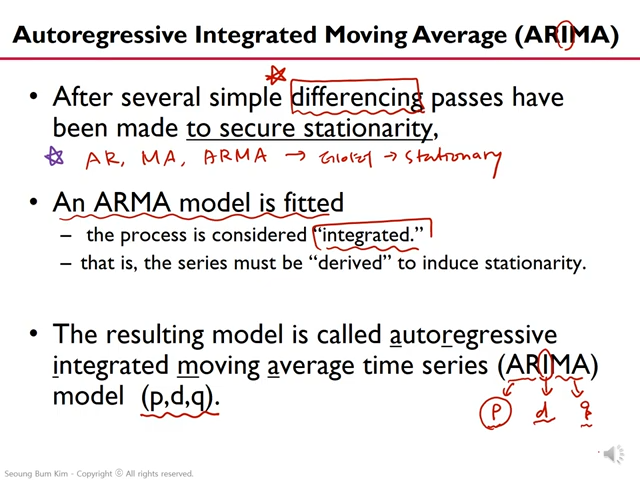
\includegraphics[width=.45\textwidth]{3ARIMA_1}
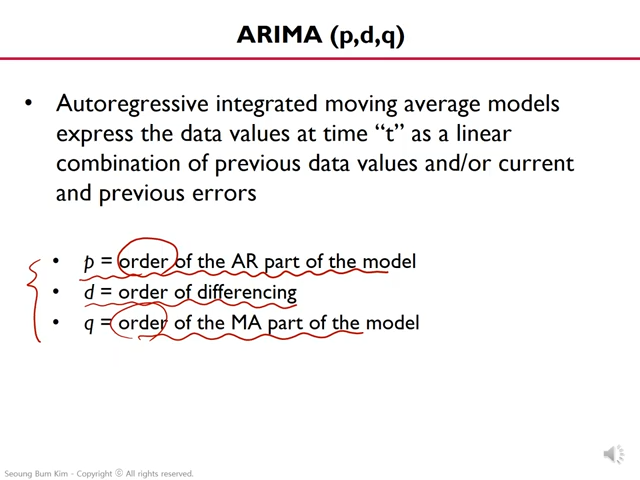
\includegraphics[width=.45\textwidth]{3ARIMA_2}
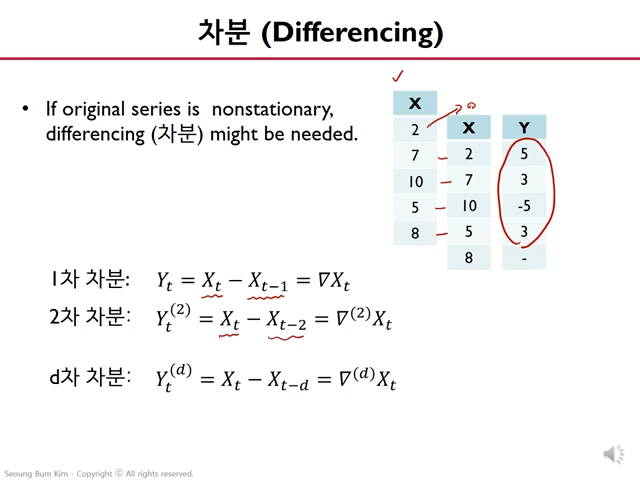
\includegraphics[width=.45\textwidth]{3ARIMA_3}
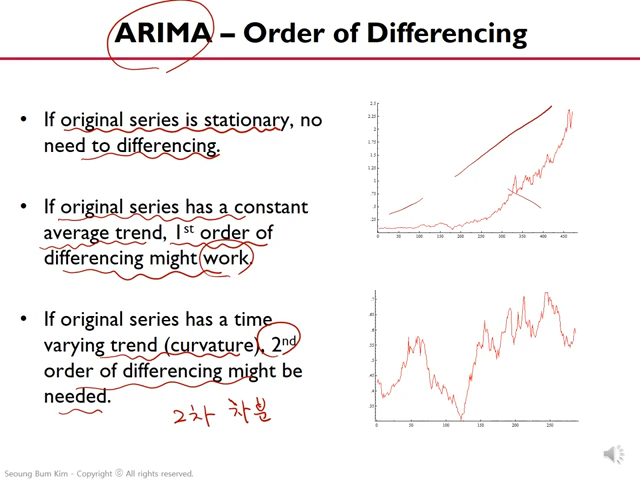
\includegraphics[width=.45\textwidth]{3ARIMA_4}
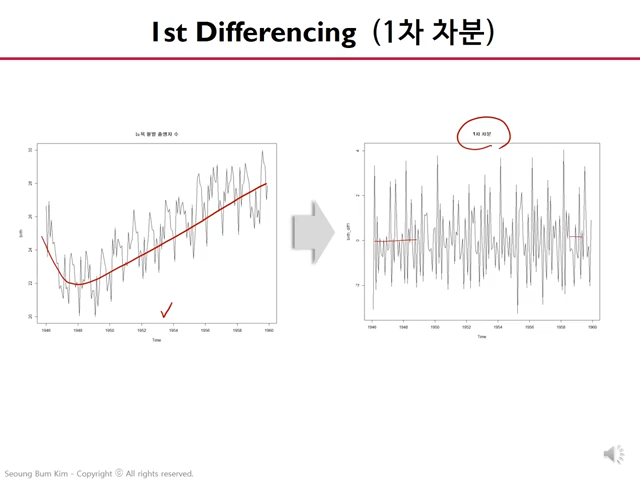
\includegraphics[width=.45\textwidth]{3ARIMA_5}
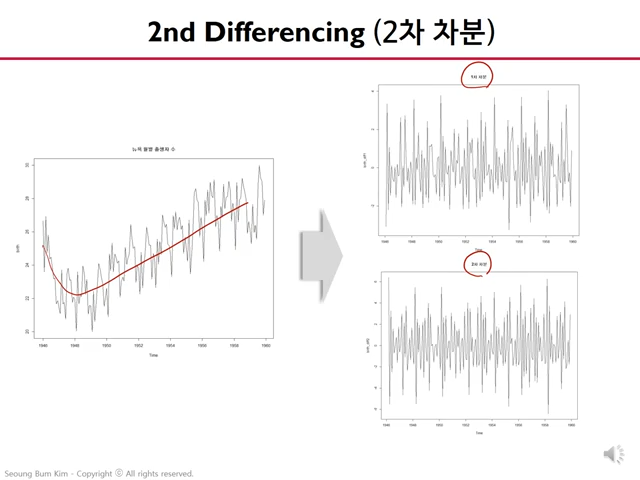
\includegraphics[width=.45\textwidth]{3ARIMA_6}
\end{center}
ARMA 모델에 차분(differencing)까지 적용하면 ARIMA(autoregressive integrated moving average model) 모델을 만들 수 있다.

여기서 차분이란, 계차수열과 같은 것을 말한다.
즉, 시계열 \(\{X_t\}\)가 주어졌을 때, 새로운 시계열 \(\{Y_t\}\)

\end{document}